\documentclass{article}
\usepackage[portuguese]{babel}
\usepackage[natbibapa]{apacite}
\bibliographystyle{apacite}
\usepackage{url}
\usepackage{pdfpages}
%\usepackage[utf8x]{inputenc}
\usepackage{amsmath}
\usepackage{graphicx}
\usepackage{listings}
\graphicspath{{images/}}
\usepackage{parskip}
\usepackage{fancyhdr}
\usepackage{vmargin}
\usepackage{float}
\usepackage{caption}
\usepackage{subcaption}
\usepackage{hyperref}
\usepackage{listings}
\usepackage{pdfpages}
\usepackage{bytefield}
\usepackage{array} 
\usepackage{xparse}
\usepackage{tikz}
\usepackage{verbatim}
\usepackage{arydshln}
\usepackage{mathtools}
\usepackage{booktabs}
\usepackage{tabulary,lipsum}
\usepackage{svg}
\usepackage{pdflscape}
\tymin=60pt
\tymax=\maxdimen
\usepackage{minted}
\usepackage[utf8]{inputenc}
\NewDocumentCommand{\codeword}{v}{%
\texttt{\textcolor{codegreen}{#1}}%
}
\setminted{
fontsize=\large,
breaklines,
breakbytoken=false,
breakautoindent=true,
baselinestretch=1.0,
framesep=2mm,
numbersep=2mm,
linenos,
frame=leftline
}

\usepackage[framed,numbered]{matlab-prettifier}
\lstset{
  style      = Matlab-editor,
  basicstyle = \fontfamily{pcr}\selectfont\footnotesize, % if you want to use Courier
}

\lstdefinelanguage{C2}[]{C}{
    morestring = [s][\color{codelaranja}]{<}{>},
}

\lstdefinestyle{mystyle}{
    backgroundcolor=\color{backcolour},   
    commentstyle=\color{codegreen},
    keywordstyle=\color{AzulTop},
    numberstyle=\tiny\color{codegray},
    stringstyle=\color{codelaranja},
    basicstyle=\ttfamily\footnotesize,
    breakatwhitespace=false,         
    breaklines=true,                 
    captionpos=b,                    
    keepspaces=true,                 
    numbers=left,                    
    numbersep=5pt,                  
    showspaces=false,                
    showstringspaces=false,
    showtabs=false,                  
    tabsize=2,
}
\usepackage[table,xcdraw]{xcolor}
\definecolor{codegreen}{rgb}{0,0.6,0}
\definecolor{codegray}{rgb}{0.5,0.5,0.5}
\definecolor{codelaranja}{rgb}{0.93,0.6,0.32}
\definecolor{backcolour}{rgb}{0.95,0.95,0.92}
\definecolor{AzulTop}{rgb}{0.3,0.55,0.94}
\definecolor{LightCyan}{rgb}{0.88,1,1}


\lstset{style=mystyle}


\newcommand{\sectionbreak}{\clearpage}

\lstset{language=bash,keywordstyle={\bfseries \color{blue}}}

\newcommand{\tikzb}[1]{\newsavebox{\#1}}

\setmarginsrb{3 cm}{2.5 cm}{3 cm}{2.5 cm}{1 cm}{1.5 cm}{1 cm}{1.5 cm}

% Para tabela
%\newcommand{\colorbitbox}[3]{%
%\rlap{\bitbox{#2}{\color{#1}\rule{\width}{\height}}}%
%\bitbox{#2}{#3}}

\definecolor{type}{HTML}{00aeff}
\definecolor{netid}{HTML}{b9a5f8}
\definecolor{nsubrede}{HTML}{fba2d3}
\definecolor{hostid}{HTML}{ffb2ae}
\definecolor{bgcolor}{HTML}{ffcda0}
\definecolor{code}{HTML}{ffa600}
\definecolor{lg}{HTML}{e6e6e6}
\definecolor{dgreen}{rgb}{0,.7,0}

\definecolor{lightcyan}{rgb}{0.84,1,1}
\definecolor{lightgreen}{rgb}{0.64,1,0.71}
\definecolor{lightred}{rgb}{1,0.7,0.71}

\setlength\parindent{24pt}

\lstdefinestyle{DOS}
{
    backgroundcolor=\color{black},
    basicstyle=\scriptsize\color{white}\ttfamily
}


\title{Relatório do Laboratório 6}								% Title
\author{} %<------------------------------------------------------								% Author
\date{\today}											% Date

\makeatletter
\let\thetitle\@title
\let\theauthor\@author
\let\thedate\@date
\makeatother

\pagestyle{fancy}
\fancyhf{}
\rhead{\theauthor}
\lhead{\thetitle}
\cfoot{\thepage}


\ifpdf
  \DeclareGraphicsRule{*}{mps}{*}{}
\fi

\begin{document}

%%%%%%%%%%%%%%%%%%%%%%%%%%%%%%%%%%%%%%%%%%%%%%%%%%%%%%%%%%%%%%%%%%%%%%%%%%%%%%%%%%%%%%%%%

\begin{titlepage}
	\centering
    \vspace*{0.2 cm}
    
\includegraphics[scale = 0.8]{logoPoli.jpg}\\[1.0 cm]	% University Logo
    \textsc{\LARGE \newline\newline Escola Politécnica da USP}\\[1.5 cm]	% University Name
    \textsc{\Large PMR3406 - Microprocessadores em Automação e Robótica}\\[0.5 cm] %Course Code     
    \textsc{\Large Turma 03 - Grupo 02}\\[0.5 cm]
	
	\rule{\linewidth}{0.2 mm} \\[0.4 cm]
	{ \huge \bfseries \thetitle}\\ 
	\rule{\linewidth}{0.2 mm} \\[1 cm]
	
	\begin{minipage}{0.5\textwidth}
		\begin{flushleft} \large

            Antônio Augusto Carnevalli\\
			Thiago Lam Braweman\\

			
			\end{flushleft}
	\end{minipage}~
	\begin{minipage}{0.5\textwidth}
            
		\begin{flushright} \large

            13682909\\
			10770502\\

		    
		    \end{flushright}
        
	\end{minipage}\\~
	\vfill
	\thedate
	
    
\end{titlepage}

%(1)-------------------------------------------------------------------------------
\section{Cálculos do PWM}

\subsection{Período do PWM}
Sendo a frequência de operação solicitada 19,53KHz, o período do PWM pode ser obtido a partir da equação:
\begin{equation}
\textit{Período do PWM} = \left[(PR2) + 1\right] \times 4 \times T_{OSC} \times (\text{Prescaler do Timer 2})
\end{equation}

Onde PR2 representa um registrador com o valor armazenado, Tosc é calculado a partir da frequência solicitada, e o Prescaler do Timer 2 pode variar entre 1:1, 1:4 ou 1:16, sendo configurado a partir dos bits $T2CKPS\langle 1{:}0 \rangle\ (\text{T2CON}\langle 1{:}0 \rangle).$

\subsection{Resolução do PWM}
O Duty Cycle do PWM é representado por um valor de 10 bits, sendo os 8-bits mais
significativos escritos no registrador CCPRxL e os 2-bits menos significativos escritos nos bits 5 e 4 do registrador CCPxCON. Pode-se calcular a largura do pulso do PWM pela seguinte equação:
\begin{equation}
    \textit{Largura do Pulso de PWM} = (\text{CCPRxL} : \text{CCPxCON}\langle 5{:}4 \rangle) \times T_{OSC} \times (\text{Prescaler do Timer 2})
\end{equation}
E o valor do Duty Cycle, em porcentagem:
\begin{equation}
\textit{Duty Cycle} = \frac{(\text{CCPRxL} : \text{CCPxCON}\langle 5{:}4 \rangle)}{4 (PR2 + 1)}
\end{equation}
CCPRxL e os bits 5 e 4 de CCPxCON podem ser alterados em qualquer instante, mas o Duty Cycle de fato só sera alterado após Timer 2 atingir o valor de PR2, ou de outra forma, quando ocorrer um período de PWM completo.
No PIC 16F886, DCxB1 e DCxB0 permitem o acesso àos bits 5 e 4 de CCPxCOM.
%(2)-------------------------------------------------------------------------------
\section{Sequência a ser programada}
\subsection{Inicialização}
Seguindo o passo a passo fornecido pela apostila de laboratório, e o código gerado para o PWM, chega-se à seguinte sequência de etapas para a inicialização (pwm\textunderscore init) correlacionadas com a sua parte do código equivalente:

\begin{enumerate}
  \item Desabilitar o pino de PWM (CCPx) setando o bit correspondente do registrador TRIS. Isto é, configurando-o para entrada.
    \begin{lstlisting}[style = Matlab-editor, language = C2]
    // 1. Desabilitando os pinos de PWM (CCPx), habilitando-os como entrada TRIS
    TRISC1 = 1; // CCP1 como entrada
    TRISC2 = 1; // CCP2 como entrada
    \end{lstlisting}
  
  \item Definir o período do PWM escrevendo no registrador \texttt{PR2}.
    \begin{lstlisting}[style = Matlab-editor, language = C2]
    // 2. Definindo o periodo da PWM no registrador PR2
    PR2 = PWM_PR2;
    \end{lstlisting}
    
  \item Configurar o módulo CCP para modo PWM carregando o registrador \texttt{CCPxCON} com os valores apropriados.
    \begin{lstlisting}[style = Matlab-editor, language = C2]
    // 3. Configurando o modulo CCP para modo PWM usando CCPxCON
    CCP1CON = 0b00001100; // Modo PWM para CCP1
    CCP2CON = 0b00001100; // Modo PWM para CCP2
    \end{lstlisting}
      
  \item Definir o \textit{Duty Cycle} do PWM escrevendo no registrador \texttt{CCPRxL} e nos bits \texttt{DCxB\textless1:0\textgreater} (\texttt{CCPxCON\textless5:4\textgreater}).
    \begin{lstlisting}[style = Matlab-editor, language = C2]
    // 4. Definindo Duty Cycle do PWM em CCPRxL e nos bits DCxB<1:0>, 0% inicial
    CCPR1L = 0;
    CCP1CONbits.DC1B = 0;

    CCPR2L = 0;
    CCP2CONbits.DC2B1 = 0;
    CCP2CONbits.DC2B0 = 0;
    \end{lstlisting}
      
  \item Configurar e disparar o Timer 2:
  \begin{enumerate}
    \item Limpar o bit do \textit{flag} de interrupção \texttt{TMR2IF} (\texttt{PIR1\textless1\textgreater});
    \item Definir o valor do prescaler do Timer 2 carregando os bits \texttt{T2CKPS\textless1:0\textgreater} (\texttt{T2CON\textless1:0\textgreater});
    \item Habilitar o Timer 2, fazendo o bit \texttt{TMR2ON} = 1 (\texttt{T2CON\textless2\textgreater}).
  \end{enumerate}
    \begin{lstlisting}[style = Matlab-editor, language = C2]
    // 5. Configurando e disparando Timer 2
    PIR1bits.TMR2IF = 0;      // Limpa flag
    T2CONbits.T2CKPS = 0b01;  // Prescaler do timer 2 como 4
    T2CONbits.TMR2ON = 1;     // Liga Timer 2
    \end{lstlisting}
    
  \item Habilitar a saída PWM depois que um novo ciclo de PWM tiver sido iniciado:
  \begin{enumerate}
    \item Esperar pelo transbordo do Timer 2 (bit \texttt{TMR2IF} = 1 (\texttt{PIR1\textless1\textgreater}));
    \item Habilitar a saída do pino de PWM (CCPx) limpando o bit correspondente do registrador \texttt{TRIS}. Isto é, configurando-o para saída.
  \end{enumerate}
    \begin{lstlisting}[style = Matlab-editor, language = C2]
    // 6. Habilitando a saida PWM depois que um novo ciclo iniciar
    while (!PIR1bits.TMR2IF); // Esperando o transbordo
    TRISCbits.TRISC2 = 0;     // CCP1 como saida (motor esquerdo)
    TRISCbits.TRISC1 = 0;     // CCP2 como saida (motor direito)
    \end{lstlisting}
      
\end{enumerate}
\subsection{Alteração do Duty Cycle do PWM}
\begin{lstlisting}[style = Matlab-editor, language = C2]
void pwm_set(int channel, int duty_cycle){
    
    // Limitando os valores para 0-100%
    if (duty_cycle < 0) duty_cycle = 0;
    if (duty_cycle > 1000) duty_cycle = 1000;
  
    switch (channel) {
        case 1: // Motor esquerdo - CCP1
            CCPR1L = (unsigned char) duty_cycle;  // Define os 8 MSBs do duty cycle de CCP1                     
            
            break;
        case 2: // Motor direito - CCP2
            CCPR2L = (unsigned char) duty_cycle;  // Define os 8 MSBs do duty cycle de CCP2  
            
            break;
        default:
            // Canal invalido, nao faz nada
            break;
        }
}
\end{lstlisting}
%(3)-------------------------------------------------------------------------------
\section{Comparação de valores de velocidade}
Nesta secção devemos calcular a velocidade do robô e relaciona-la com um valor do Duty Cycle do PWM e om isso criar um gráfico, e depois uma equação que aproxima essa relação para demais valores.
Infelizmente o grupo não conseguiu retirar as medidas durante o Laboratório, então não foi possível construir o gráfico ou a equação, mas vamos explicar como ele e a formula da velocidade deveriam ser criados.\par

\subsection{Cálculo da velocidade}
Com o encoder e o diâmetro das rodas é possível calcular a velocidade que elas giram. Sabemos que uma volta completa de uma das rodas representa 12 pulsos em uma das fases do encoder, e a roda têm diâmetro de 42 mm, assim temos que o perímetro da roda ($P = \pi d $) é de aproximadamente \textbf{131,95 mm}, arredondando para um valor inteiro temos o resultado de \textbf{132 mm}.\par

A partir do número de pulsos por volta \textbf{12} e do perímetro de \textbf{132 mm} concluímos que cada pulso corresponde a aproximadamente \textbf{11 mm}  ou \textbf{11 mm/pulso}. Com isso temos as ferramentas para o cálculo da velocidade, em um intervalo de tempo determinado contamos o número de pulsos e usamos a conversão de pulsos por milímetro obtendo finalmente a velocidade conforme o exemplo abaixo.\par

\begin{align*}
    Tempo &= 2 &[s]\\
    \\
    Pulsos &= 48 \\
    \\
    Distancia &= 11 * Pulsos &[mm] \\
    Distancia &= 528 &[mm]\\
    \\
    Velocidade &= Distancia / Tempo &[mm/s]\\
    Velocidade &= 264 &[mm/s]\\
\end{align*}

Implementado no PIC esse cálculo e utilizando o LCD podemos ver a velocidade das rodas a todo momento, com o osciloscópio do laboratório podemos verificar simultaneamente o sinal do PWM no formato da imagem \ref{fig:DutyCycle} (retirada da página 44 da apostila), assim verificando o Duty Cycle porcentual. Devemos repetimos essa medição 5 vezes variando o sinal do PWM gerando a tabela incompleta \ref{fig:speed}.\par

\begin{figure}[H]
    \centering
    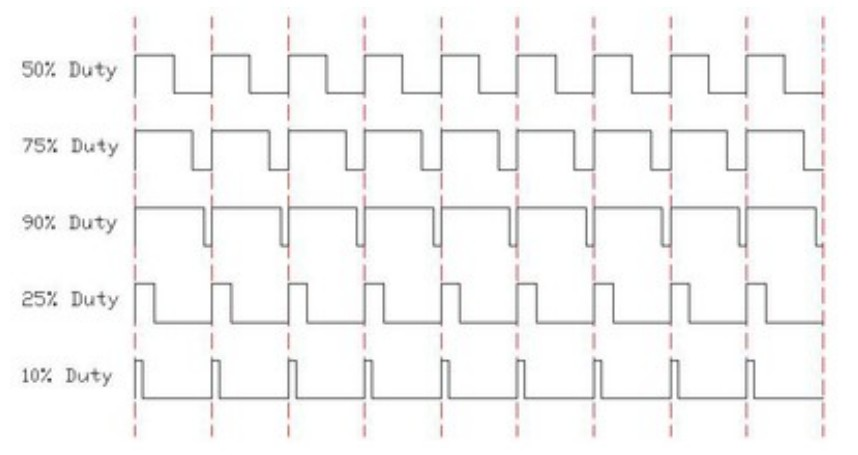
\includegraphics[width = .8\linewidth]{images/SinalPWM.jpg}
    \caption{Sinais do PWM com relação ao Duty Cycle}
    \label{fig:DutyCycle}
\end{figure}

\begin{figure}[H]
    \centering
    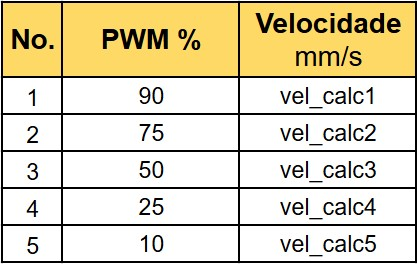
\includegraphics[width = .4\linewidth]{images/tabelavelocidade.jpg}
    \caption{Tabela do porcentual do Duty Cycle pela velocidade medida}
    \label{fig:speed}
\end{figure}


\subsection{Gráfico obtido}


Com os dados da tabela \ref{fig:speed} poderíamos ter criado uma um gráfico da relação \textbf{PWD\% x Velocidade} do formato da figura \ref{fig:grafPWMvel} abaixo.

\begin{figure}[H]
    \centering
    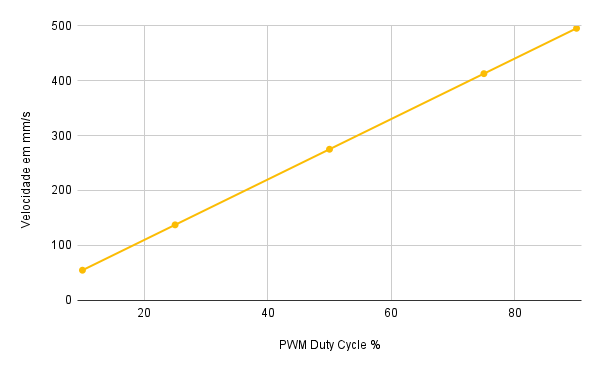
\includegraphics[width = .8\linewidth]{images/SpeedXPWM.png}
    \caption{Gráfico porcentagem de PWM com velocidade do motor}
    \label{fig:grafPWMvel}
\end{figure}

\subsection{Porcentagem de PWM em mm/s}

Com base nos dados do gráfico podemos aproximar uma função com entrada o percentual do Duty Cycle do PWM e com saída a velocidade do robô.

\begin{equation*}
    V(PWM_\%)  =  PWM_\%
\end{equation*}

\subsection{Velocidade medida X velocidade calculada}

Com a equação definida deveríamos comparar outros valores do Duty Cycle do PWM e ver se a diferença com as velocidades reais.
%-------------------------------------------------------------------------------
\section{Código fonte}

\subsection*{PWM modificado para o Lab}
As funções \codeword{pwm_on()}, \codeword{pwm_off()} e \codeword{pwm_output_control()} foram removidas, e a função \codeword{pwm_set(int channel, int duty_cycle)} foram implementadas.
\inputminted{c}{code/pwm.c}
\newpage

\subsection*{Medir velocidade e PWM pela distância}
O código cálcula a velocidade das rodas e ajusta a velocidade delas pela proximidade de outros obstáculos até um certo limite \codeword{DIST_THRESHOLD}.
\inputminted{c}{code/main.c}


\end{document}